\input{../latexSetup}

\usepackage{tikz}
\usetikzlibrary{arrows.meta, decorations.markings}
\usepackage{nicefrac}
\usepackage{amssymb}

\lhead{\Large 33-211}
\chead{\Large Physics 3 : Modern Essentials}
\rhead{\Large Lecture 3}

\begin{document}
\thispagestyle{fancy}

\begin{center}
  {\huge \textbf{The Need For Change}}
\end{center}

% ============================================================
\section*{Why Aren't Galilean Transforms Good Enough?}

Bunch of good reasons:
\begin{itemize}
  \item E\&M / Maxwell's equations (last time) \checkmark
  \item Determinism \checkmark
  \item General Coordinate Transformations (this lecture, bonus derivation)
  \item Philosophy --- Einstein's main motivation (+EM) \hfill \textit{(Next time)}
  \item \textbf{Experiment!} \hfill \textit{(this lecture)}
\end{itemize}

% ============================================================
\section*{The Experiment: Michelson \& Morley}

\textbf{Early 20\textsuperscript{th} C context:} All waves were known to propagate in some
``medium'' (water, sound, etc.).

Light is a wave! (e.g.\ double-slit experiment / Maxwell's equations.)
$\Rightarrow$ There must be an associated medium: the \textbf{``Ether''}.

Maxwell's equations $\Rightarrow$ light waves move at
\[
  c = \frac{1}{\sqrt{\varepsilon_0 \mu_0}} \approx 3\times10^8\;\text{m/s}
  \quad (1\;\text{ft/ns} \text{ or } 30\;\text{cm/ns})
\]
\emph{with respect to the ether}.

The Earth moves at $\sim 30\;\text{km/s}$. Because it moves in a circle, it
can't always align its velocity with the ether wind.

\medskip
\textbf{Question:} Can we detect the change in speed of light due to Earth's motion?

\[
  v_e \sim 30\;\frac{\text{km}}{\text{s}}, \qquad
  c \sim 3\times10^8\;\text{m/s} \sim 3\times10^5\;\frac{\text{km}}{\text{s}}
\]
\[
  \frac{v_e}{c} \sim 10^{-4}
\]

% ============================================================
\section*{The Interferometer}

\textbf{Idea:} Compare the time of flight for light traveling in
\emph{different} directions (parallel vs.\ perpendicular to the ether wind).

\begin{center}
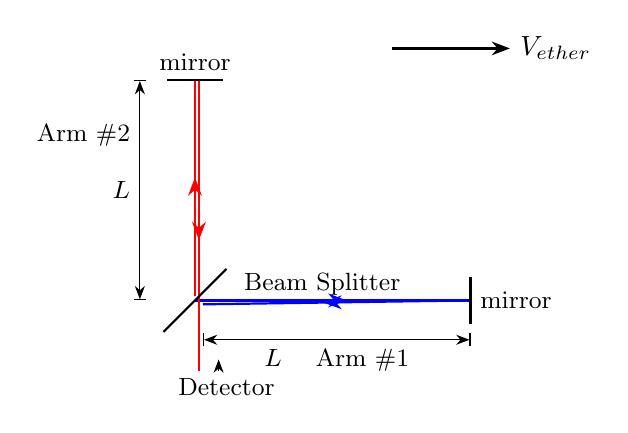
\begin{tikzpicture}[scale=1.0, >=Stealth,
    ray/.style={thick, postaction={decorate,
      decoration={markings, mark=at position 0.55 with {\arrow{Stealth}}}}}]

  % Ether velocity arrow (top right)
  \draw[->, thick] (2.5, 3.2) -- (4.0, 3.2) node[right] {$V_{\text{ether}}$};

  % --- Horizontal arm (Arm #1) ---
  % Beam path: right and return (blue)
  \draw[ray, blue] (0, 0) -- (3.5, 0);   % outgoing
  \draw[ray, blue] (3.5, 0) -- (0.1,-0.05); % returning (slight offset for clarity)
  % Right mirror
  \draw[thick] (3.5,-0.3) -- (3.5, 0.3);
  \node[right, font=\small] at (3.5, 0) {mirror};
  % Arm #1 label and length
  \draw[|<->|, thin] (0.1,-0.5) -- (3.5,-0.5);
  \node[below, font=\small] at (1.8,-0.5) {$L$ \quad Arm \#1};

  % --- Vertical arm (Arm #2) ---
  % Beam path: up and return (red)
  \draw[ray, red]  (0, 0.05) -- (0, 2.8); % outgoing (slight offset)
  \draw[ray, red]  (0.05, 2.8) -- (0.05,-0.9); % returning + to detector
  % Top mirror
  \draw[thick] (-0.35, 2.8) -- (0.35, 2.8);
  \node[above, font=\small] at (0, 2.8) {mirror};
  % Arm #2 label and length
  \draw[|<->|, thin] (-0.7, 0) -- (-0.7, 2.8);
  \node[left, font=\small] at (-0.7, 1.4) {$L$};
  \node[left, font=\small] at (-0.7, 2.1) {Arm \#2};

  % --- Beam splitter (diagonal line at origin) ---
  \draw[thick] (-0.4,-0.4) -- (0.4, 0.4);
  \node[right, font=\small] at (0.5, 0.2) {Beam Splitter};

  % --- Detector (below) ---
  \node[font=\small] at (0.4, -1.1) {Detector};
  \draw[->, thin] (0.3,-0.9) -- (0.3,-0.75);

\end{tikzpicture}
\end{center}

\subsection*{Arm \#1 (parallel to ether motion)}

Light travels distance $L$ with ether, then $L$ against it:
\[
  t_1 = \frac{L}{c+v} + \frac{L}{c-v}
      = \frac{L}{c}\left[\frac{1}{1+\nicefrac{v}{c}} + \frac{1}{1-\nicefrac{v}{c}}\right]
\]

Define $\beta \equiv v/c \ll 1$:
\[
  t_1 = \frac{L}{c}\left[\frac{1}{1+\beta} + \frac{1}{1-\beta}\right]
      = \frac{L}{c}\Bigl[(1-\beta+\beta^2+\mathcal{O}(\beta^3))
                       + (1+\beta+\beta^2+\mathcal{O}(\beta^3))\Bigr]
\]
\[
  \boxed{t_1 = \frac{2L}{c}\Bigl[1 + \beta^2 + \mathcal{O}(\beta^3)\Bigr]}
\]

\subsection*{Arm \#2 (perpendicular to ether motion)}

Light must travel at an angle to reach the mirror (which is moving with the Earth).
The effective speed is $\sqrt{c^2-v^2}$:
\[
  t_2 = \frac{L}{\sqrt{c^2-v^2}} + \frac{L}{\sqrt{c^2-v^2}}
      = \frac{2L}{c}\left(1 + \tfrac{1}{2}\beta^2 + \mathcal{O}(\beta^3)\right)
\]

\subsection*{Time Difference}

\[
  \Delta t = t_2 - t_1
  = \frac{2L}{c}\Bigl[\bigl(1+\tfrac{1}{2}\beta^2+\mathcal{O}(\beta^3)\bigr)
                     - \bigl(1+\beta^2+\mathcal{O}(\beta^3)\bigr)\Bigr]
  = \frac{2L}{c}\left[-\tfrac{1}{2}\beta^2\right] + \mathcal{O}(\beta^3)
\]
\[
  \boxed{\Delta t = -\frac{Lv^2}{c^3}}
\]

(The sign shows Arm \#2 is faster; only $|\Delta t|$ matters for fringe counting.)

% ============================================================
\section*{Detection via Interference}

The tiny wavelength of light allows us to probe tiny $\Delta t$ by looking for
\textbf{interference fringes}.

\begin{center}
% x=0.4cm sets the coordinate unit so many-cycle waves fit without stretching text nodes.
% omega=1.5 => period T = 2pi/1.5 ~ 4.19 coord-units = 1.68 cm displayed
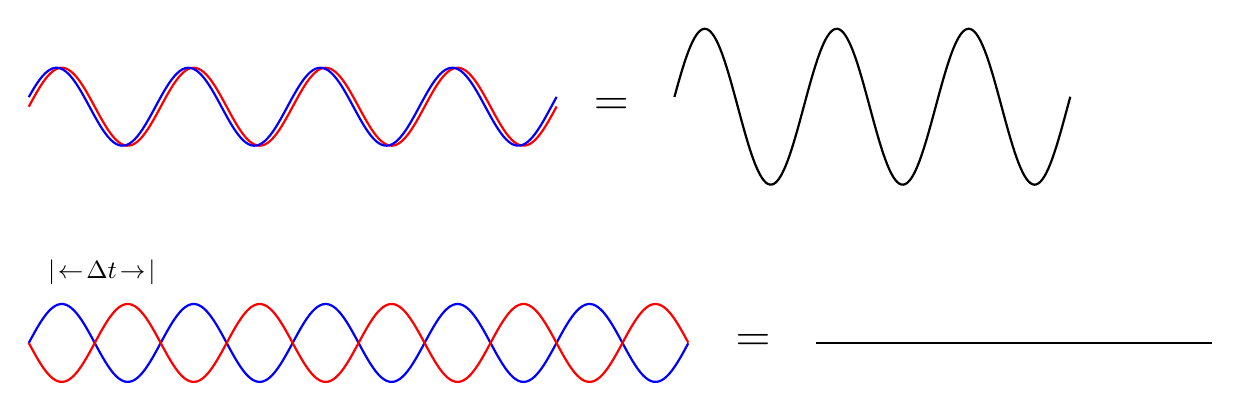
\begin{tikzpicture}[x=0.4cm, y=1.1cm, >=Stealth]

  % --- TOP: nearly in phase (0.25 rad offset) -> constructive ---
  % 4 cycles: domain 0 .. 4T ~ 16.76
  \draw[red,  thick, domain=0:16.76, samples=200]
    plot (\x, {0.45*sin(1.5*\x r)});
  \draw[blue, thick, domain=0:16.76, samples=200]
    plot (\x, {0.45*sin(1.5*\x r + 14.3)});   % 14.3 deg = 0.25 rad (small visible offset)
  \node[font=\LARGE] at (18.5, 0) {$=$};
  % Result: ~doubled amplitude, 3 cycles
  \draw[black, thick, domain=20.5:33.07, samples=200]
    plot (\x, {0.9*sin(1.5*(\x - 20.5) r + 7.2)});  % 7.2 deg = 0.125 rad

  % --- BOTTOM: pi shift -> destructive ---
  % 5 cycles: domain 0 .. 5T ~ 20.94
  \begin{scope}[yshift=-3.0cm]
    % Small text label at top-left, matching the handwritten |<- Dt ->| style
    \node[font=\small, anchor=west] at (0.3, 0.82)
      {$|\!\leftarrow\!\Delta t\!\rightarrow\!|$};
    \draw[blue, thick, domain=0:20.94, samples=250]
      plot (\x, {0.45*sin(1.5*\x r)});
    \draw[red,  thick, domain=0:20.94, samples=250]
      plot (\x, {0.45*sin(1.5*\x r + 180)});   % 180 deg = pi rad (half-period shift)
    \node[font=\LARGE] at (23, 0) {$=$};
    % Result: flat line, same displayed length as top result
    \draw[black, thick] (25, 0) -- (37.57, 0);
  \end{scope}

\end{tikzpicture}
\end{center}

The phase shift between the two arms:
\[
  \Delta\phi \sim \frac{c\,\Delta t}{\lambda}
             \sim \frac{L}{\lambda}\left(\frac{v}{c}\right)^2
\]

Plugging in MM's numbers ($L \approx 10\;\text{m}$, $\lambda \approx 590\;\text{nm}$,
$v_e/c \sim 10^{-4}$):
\[
  \Delta\phi = 4\pi\,\frac{10\;\text{m}}{590\;\text{nm}}\,(10^{-4})^2
             \approx 2.1 \approx 0.3\times 2\pi
             \quad\Rightarrow\quad \tfrac{1}{3}\ \text{of a fringe}
\]

\begin{tcolorbox}
  \textbf{Easily observable --- but not seen!}
\end{tcolorbox}

% ============================================================
\section*{General Coordinate Transformations}

\subsection*{Setup}

Motivated by the MM result (and the other reasons listed above), we look for the
\emph{most general} linear coordinate transform between two reference frames
moving with relative velocity $v$.

\subsubsection*{Step 1 --- Assume linearity}

\[
  x = ax' + bt', \qquad t = ex' + ft'
  \qquad\text{or}\qquad
  \begin{pmatrix}x\\t\end{pmatrix} = \begin{pmatrix}a&b\\e&f\end{pmatrix}
  \begin{pmatrix}x'\\t'\end{pmatrix}
\]
where $(a,b,e,f)$ are unknown functions of $v$.

\subsubsection*{Step 2 --- Impose relative velocity}

When $x'=0$: the origin of $F'$ moves at speed $v$ in $F$, so $x = vt$:
\[
  \begin{pmatrix}x\\t\end{pmatrix}
  = \begin{pmatrix}a&b\\e&f\end{pmatrix}\begin{pmatrix}0\\t'\end{pmatrix}
  = \begin{pmatrix}bt'\\ft'\end{pmatrix}
  \quad\Rightarrow\quad \frac{x}{t} = \frac{b}{f} = v
  \quad\Rightarrow\quad b = vf
\]

So the transform becomes:
\[
  \begin{pmatrix}x\\t\end{pmatrix}
  = f\begin{pmatrix}a/f & v \\ e/f & 1\end{pmatrix}
  \begin{pmatrix}x'\\t'\end{pmatrix}
\]

\subsubsection*{Step 3 --- Symmetry of the two frames}

When $x=0$: the origin of $F$ moves at speed $-v$ in $F'$, so $x' = -vt'$:
\[
  \begin{pmatrix}0\\t\end{pmatrix}
  = f\begin{pmatrix}a/f & v \\ e/f & 1\end{pmatrix}
    \begin{pmatrix}-vt'\\t'\end{pmatrix}
  = f\begin{pmatrix} (a/f)(-vt') + vt' \\ (e/f)(-vt') + t' \end{pmatrix}
  = f\begin{pmatrix} vt'(1-a/f) \\ \cdots \end{pmatrix}
\]

For the top component to vanish: $1 - a/f = 0 \Rightarrow a = f$.

So the \textbf{general C.T.} takes the form:
\[
  \begin{pmatrix}x\\t\end{pmatrix}
  = a\begin{pmatrix}1 & v \\ e/a & 1\end{pmatrix}
  \begin{pmatrix}x'\\t'\end{pmatrix}
\]

\subsubsection*{Step 4 --- Impose group structure}

Two successive transforms $v_1$ then $v_2$:
\[
  \begin{pmatrix}x''\\t''\end{pmatrix}
  \xrightarrow{v_1}
  \begin{pmatrix}x'\\t'\end{pmatrix}
  \xrightarrow{v_2}
  \begin{pmatrix}x\\t\end{pmatrix}
\]

\begin{align*}
  \begin{pmatrix}x\\t\end{pmatrix}
  &= a(v_2)\begin{pmatrix}1&v_2\\[3pt]\frac{e}{a}(v_2)&1\end{pmatrix}
    \cdot
    a(v_1)\begin{pmatrix}1&v_1\\[3pt]\frac{e}{a}(v_1)&1\end{pmatrix}
    \begin{pmatrix}x''\\t''\end{pmatrix} \\[6pt]
  &= a(v_2)a(v_1)
    \begin{pmatrix}
      1+\frac{e}{a}(v_1)\cdot v_2 & v_1+v_2 \\[4pt]
      \frac{e}{a}(v_1)+\frac{e}{a}(v_2) & 1+\frac{e}{a}(v_2)\cdot v_1
    \end{pmatrix}
    \begin{pmatrix}x''\\t''\end{pmatrix}
\end{align*}

This must equal $T(v_c)$ acting on $(x'',t'')$.
For the diagonal elements to be equal (required for a single combined transform):
\[
  1 + \tfrac{e}{a}(v_1)\cdot v_2 = 1 + \tfrac{e}{a}(v_2)\cdot v_1
  \quad\Rightarrow\quad
  \frac{1}{v_1}\frac{e}{a}(v_1) = \frac{1}{v_2}\frac{e}{a}(v_2)
\]

By separation of variables, both sides equal a constant $g$ (free, independent of $v$):
\[
  \frac{1}{v}\frac{e}{a}(v) = g
  \quad\Rightarrow\quad
  \frac{e}{a}(v) = gv
\]

So the general C.T.\ is:
\[
  \begin{pmatrix}x\\t\end{pmatrix}
  = a\begin{pmatrix}1 & v \\ gv & 1\end{pmatrix}
  \begin{pmatrix}x'\\t'\end{pmatrix}
\]

\textbf{Note on dimensions:}
$[g] = [t]/[x]^2 \cdot [x]/[t] = 1/[v]^2$, so we write $g = 1/v_*^2$
for some characteristic speed $v_*$.

\subsubsection*{Step 5 --- Find $a(v)$}

Impose the round-trip: $(x,t) \xrightarrow{v} (x',t') \xrightarrow{-v} (x,t)$:

\begin{align*}
  \begin{pmatrix}x\\t\end{pmatrix}
  &= a(-v)\begin{pmatrix}1&-v\\[3pt]-v/v_*^2&1\end{pmatrix}
    \cdot
    a(v)\begin{pmatrix}1&v\\[3pt]v/v_*^2&1\end{pmatrix}
    \begin{pmatrix}x\\t\end{pmatrix} \\[6pt]
  &= a(-v)\,a(v)
    \begin{pmatrix}1-v^2/v_*^2 & 0 \\ 0 & 1-v^2/v_*^2\end{pmatrix}
    \begin{pmatrix}x\\t\end{pmatrix}
\end{align*}

This must equal the identity, so:
\[
  a(-v)\,a(v) = \frac{1}{1-v^2/v_*^2}
\]

Symmetry of space $\Rightarrow a(v) = a(|v|)$, hence $a(-v) = a(v)$ and:
\[
  (a(v))^2 = \frac{1}{1-v^2/v_*^2}
  \quad\Rightarrow\quad
  \boxed{a(v) = \frac{1}{\sqrt{1-v^2/v_*^2}} \equiv \gamma_v}
\]

\subsubsection*{Result: General Coordinate Transform}

Parameterized by the free constant $v_*$:

\begin{tcolorbox}
\[
  \begin{pmatrix}x\\t\end{pmatrix}
  = \frac{1}{\sqrt{1-\bigl(\frac{v}{v_*}\bigr)^2}}
    \begin{pmatrix}1 & v \\[6pt] \dfrac{v}{v_*^2} & 1\end{pmatrix}
  \begin{pmatrix}x'\\t'\end{pmatrix}
\]
\end{tcolorbox}

When $v_*\to\infty$, the prefactor $\to 1$ and $v/v_*^2 \to 0$, recovering the
\textbf{Galilean Transform}:
$\begin{pmatrix}x\\t\end{pmatrix} = \begin{pmatrix}1&v\\0&1\end{pmatrix}\begin{pmatrix}x'\\t'\end{pmatrix}$.

% ============================================================
\section*{What is $v_*$?}

Suppose something moves at speed $v_*$ in the primed frame: $x' = v_*\, t'$.

In unprimed coordinates:
\[
  \begin{pmatrix}x\\t\end{pmatrix}
  = \gamma_{v_*}\begin{pmatrix}1&v\\[4pt]v/v_*^2&1\end{pmatrix}
    \begin{pmatrix}v_*\,t'\\t'\end{pmatrix}
  = \gamma_{v_*}\begin{pmatrix}(v_*+v)\,t'\\[4pt]\frac{v}{v_*}\,t'+t'\end{pmatrix}
\]

\[
  \frac{x}{t} = \frac{v_*+v}{\frac{v}{v_*}+1}
              = \frac{v_*+v}{\frac{v+v_*}{v_*}}
              = v_*
\]

So anything moving at $v_*$ in one frame moves at $v_*$ in all frames.
$v_*$ is simultaneously:
\begin{itemize}
  \item the \textbf{maximum speed} (no frame transformation can exceed it)
  \item a \textbf{coordinate invariant}
\end{itemize}

% ============================================================
\section*{The Invariant Interval}

\textbf{Finally, note} the quantity $v_*^2 t^2 - x^2$ is invariant:

\begin{align*}
  v_*^2 t^2 - x^2
  &= v_*^2\!\left(\frac{\frac{v}{v_*^2}x'+t'}{\sqrt{1-(v/v_*)^2}}\right)^{\!2}
   - \left(\frac{x'+vt'}{\sqrt{1-(v/v_*)^2}}\right)^{\!2} \\[6pt]
  &= \frac{1}{1-(v/v_*)^2}
     \Bigl[
       \bigl(\tfrac{v}{v_*}x'+v_*t'\bigr)^2 - (x'+vt')^2
     \Bigr] \\[6pt]
  &= \frac{1}{1-(v/v_*)^2}
     \Biggl[
       \frac{v^2}{v_*^2}x'^2 + 2vx't' + v_*^2 t'^2
       - x'^2 - 2vx't' - v^2 t'^2
     \Biggr] \\[6pt]
  &= \frac{1}{1-(v/v_*)^2}
     \left[
       (v_*^2 - v^2)t'^2 + \left(\frac{v^2}{v_*^2}-1\right)x'^2
     \right] \\[6pt]
  &= \frac{1}{1-(v/v_*)^2}
     \left[
       (v_*^2-v^2)t'^2 - \left(1-\frac{v^2}{v_*^2}\right)x'^2
     \right] \\[6pt]
  &= v_*^2 t'^2 - x'^2
\end{align*}

\begin{tcolorbox}
\[
  v_*^2\,t^2 - x^2 = v_*^2\,t'^2 - x'^2 \qquad \textbf{(Invariant Interval)}
\]
\end{tcolorbox}

\textbf{P.P.S.}\ When $v_*\to\infty$ we recover the Galilean transform:
\[
  \begin{pmatrix}x\\t\end{pmatrix}
  = \underbrace{\frac{1}{\sqrt{1-v^2/v_*^2}}}_{\to\;1}
    \begin{pmatrix}1 & v \\[4pt] v/v_*^2 & 1\end{pmatrix}
    \begin{pmatrix}x'\\t'\end{pmatrix}
  \;\xrightarrow{v_*\to\infty}\;
  \begin{pmatrix}1&v\\0&1\end{pmatrix}
  \begin{pmatrix}x'\\t'\end{pmatrix}
\]
i.e.\ $x = x' + vt'$, $\;t = t'$.

\end{document}
